\documentclass[]{article}
\usepackage{times}
\usepackage{amssymb,amsmath}
\usepackage{ifxetex,ifluatex}
\usepackage{fixltx2e} % provides \textsubscript
\ifnum 0\ifxetex 1\fi\ifluatex 1\fi=0 % if pdftex
  \usepackage[T1]{fontenc}
  \usepackage[utf8]{inputenc}
\else % if luatex or xelatex
  \ifxetex
    \usepackage{mathspec}
  \else
    \usepackage{fontspec}
  \fi
  \defaultfontfeatures{Ligatures=TeX,Scale=MatchLowercase}
\fi
% use upquote if available, for straight quotes in verbatim environments
\IfFileExists{upquote.sty}{\usepackage{upquote}}{}
% use microtype if available
\IfFileExists{microtype.sty}{%
\usepackage{microtype}
\UseMicrotypeSet[protrusion]{basicmath} % disable protrusion for tt fonts
}{}
% \usepackage{hyperref}
% % \hypersetup{unicode=true,
% %             pdftitle={Pharmacist responsibilities when selling complementary medicines},
% % %             pdfauthor={Adam La Caze (UQ); Amber Salman Popattia (UQ); Laetitia Hattingh (Griffith)},
% % % %             pdfborder={0 0 0},
% %             breaklinks=true}

\usepackage[colorlinks=true, urlcolor=blue, linkcolor=black, citecolor=blue, pdfauthor={Adam La Caze}]{hyperref}
\usepackage{url}

\urlstyle{same}  % don't use monospace font for urls

\usepackage[style=authoryear]{biblatex}

\addbibresource{Presentation.bib}
\usepackage{graphicx,grffile}
\makeatletter
\def\maxwidth{\ifdim\Gin@nat@width>\linewidth\linewidth\else\Gin@nat@width\fi}
\def\maxheight{\ifdim\Gin@nat@height>\textheight\textheight\else\Gin@nat@height\fi}
\makeatother
% Scale images if necessary, so that they will not overflow the page
% margins by default, and it is still possible to overwrite the defaults
% using explicit options in \includegraphics[width, height, ...]{}
\setkeys{Gin}{width=\maxwidth,height=\maxheight,keepaspectratio}
\IfFileExists{parskip.sty}{%
\usepackage{parskip}
}{% else
\setlength{\parindent}{0pt}
\setlength{\parskip}{6pt plus 2pt minus 1pt}
}
\setlength{\emergencystretch}{3em}  % prevent overfull lines
\providecommand{\tightlist}{%
  \setlength{\itemsep}{0pt}\setlength{\parskip}{0pt}}
\setcounter{secnumdepth}{0}
% Redefines (sub)paragraphs to behave more like sections
\ifx\paragraph\undefined\else
\let\oldparagraph\paragraph
\renewcommand{\paragraph}[1]{\oldparagraph{#1}\mbox{}}
\fi
\ifx\subparagraph\undefined\else
\let\oldsubparagraph\subparagraph
\renewcommand{\subparagraph}[1]{\oldsubparagraph{#1}\mbox{}}
\fi

%%% Use protect on footnotes to avoid problems with footnotes in titles
\let\rmarkdownfootnote\footnote%
\def\footnote{\protect\rmarkdownfootnote}


  \title{Pharmacist responsibilities when selling complementary medicines}
    \author{Adam La Caze (UQ) \\ Amber Salman Popattia (UQ) \\ Laetitia Hattingh (Griffith)}
      \date{\today}

\usepackage{helvet}
\renewcommand\familydefault{\sfdefault} 

\def\UrlBreaks{\do\/\do-}

\usepackage{tcolorbox}
\tcbset{colback=white,colframe=blue!75}
\usepackage{comment}
\specialcomment{note}{\begin{tcolorbox}}{\end{tcolorbox}}

\begin{document}
\maketitle

\subsection{Ethics and complementary
medicines}\label{ethics-and-complementary-medicines}

\begin{itemize}
\item
  There is surprisingly little detailed ethical debate regarding the
  sale of complementary medicines in pharmacy
  \autocites{SalmanPopattia2018}{Ung2017}
\item
  There is a tendency in the literature to raise ethical conflicts
  without seeking to resolve these conflicts (e.g.~between business
  interests and evidence-based practice)
\item
  While principle-based ethics is often implied, a theoretical basis for
  ethical decision-making is rarely articulated
\end{itemize}

\subsection{A framework for pharmacist responsibilities when selling
complementary
medicines}\label{a-framework-for-pharmacist-responsibilities-when-selling-complementary-medicines}

\begin{enumerate}
\def\labelenumi{\arabic{enumi}.}
\item
  Principle-based ethics provides the theoretical foundation for the
  framework \autocite{Beauchamp2012}
\item
  \emph{Public health argument} for pharmacists selling complementary
  medicines
\item
  The responsibilities pharmacists need to fulfil when selling and
  recommending complementary medicines in order to meet their
  obligations to the public
\end{enumerate}

\subsection{Responsibilities}\label{responsibilities}

\begin{enumerate}
\def\labelenumi{\arabic{enumi}.}
\item
  Pharmacists should provide evidence-based recommendations to consumers
  regarding complementary medicines
\item
  Pharmacists should train all staff in a pharmacy and ensure that they
  provide evidence-based recommendations regarding complementary
  medicines and seek advice of a pharmacist when required
\item
  When providing advice, pharmacists should provide sufficient
  information for consumers to make informed decisions regarding
  complementary medicines
\end{enumerate}

\subsection{}\label{section}

\begin{enumerate}
\def\labelenumi{\arabic{enumi}.}
\setcounter{enumi}{3}
\item
  Pharmacists should setup the pharmacy so that consumers are provided
  an offer of advice from a pharmacist and pharmacists are available to
  provide that advice
\item
  Pharmacists must be vigilant for complementary medicine harm and
  intervene if risk of harm is significant
\end{enumerate}

\subsection{Aim}\label{aim}

Evaluate the acceptability and feasibility of the proposed ethical
framework for the sale of complementary medicines in community
pharmacies

\subsection{Methods}\label{methods}

\begin{itemize}
\item
  Australian community pharmacists were invited to participate in online
  focus groups in September and October 2019
\item
  Pharmacists were recruited using social media, professional
  organisations, and communication through the professional networks of
  key community pharmacy banner groups (e.g.~Terry White Chemmart, Good
  Price Pharmacy Warehouse, Chemist Warehouse, Amcal, Guardian,
  \ldots{})
\end{itemize}

\subsection{}\label{section-1}

\begin{itemize}
\item
  Focus group methods were modified for the online environment (Zoom
  videoconference) \autocites{Basch1987}{Knodel1993}{Gaiser2017}
\item
  Semi-structured one-on-one interviews were conducted when focus groups
  were not possible
\item
  Participants received the ethical framework prior to the workshop and
  were asked to complete a short pre-workshop survey
\item
  Focus group and interviews were video and audio recorded and
  transcribed verbatim then inductively coded and themes identified and
  refined using thematic analysis \autocite{Braun2016}
\end{itemize}

\subsection{Results \& Discussion}\label{results-discussion}

\begin{itemize}
\item
  Seventeen community pharmacists participated in 4 focus groups and 6
  individual interviews
\item
  The workshops contained 2--4 participants and went from 29 to 68
  minutes in duration (median 42.5 minutes)
\item
  The duration of the interviews ranged from 17 to 34 minutes (median 21
  minutes)
\end{itemize}

\subsection{Demographics}\label{demographics}

\begin{figure}
\centering
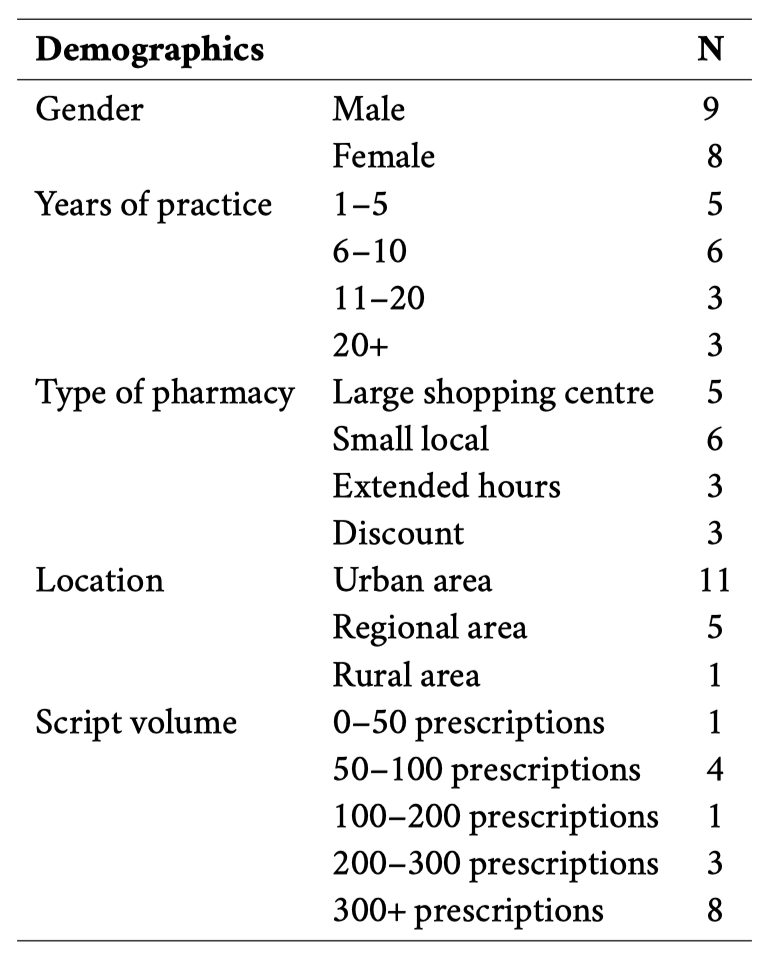
\includegraphics[width=0.50000\textwidth]{files/demo.png}
\caption{}
\end{figure}

\subsection{Theme 1: Approach to complementary medicines
(reactive--proactive)}\label{theme-1-approach-to-complementary-medicines-reactiveproactive}

\ldots{}you feel a lot \textbf{more secure at the back counter} or in a
dispensary than you do out in the vitamin section. (D5P8)

Pharmacists are becoming more involved than before. People are trusting
pharmacists more. They always check their complementary medicine. (D1P1)

\subsection{Theme 2: Approach to
evidence}\label{theme-2-approach-to-evidence}

{[}W{]}e shouldn't just be selling things because someone \ldots{} says,
``Oh, this turmeric is great for the sake of curing cancer.'' I think
\textbf{there has to be some level of evidence\ldots{}} (D4P5)

\ldots{}{[}this{]} is where \textbf{placebo effects} comes in. So hey,
if it's not doing them any harm and they think it's better for them and
they're going on in their life and happy days, you just let them go.
(D5P7)

\subsection{Variation within themes}\label{variation-within-themes}

\begin{figure}
\centering
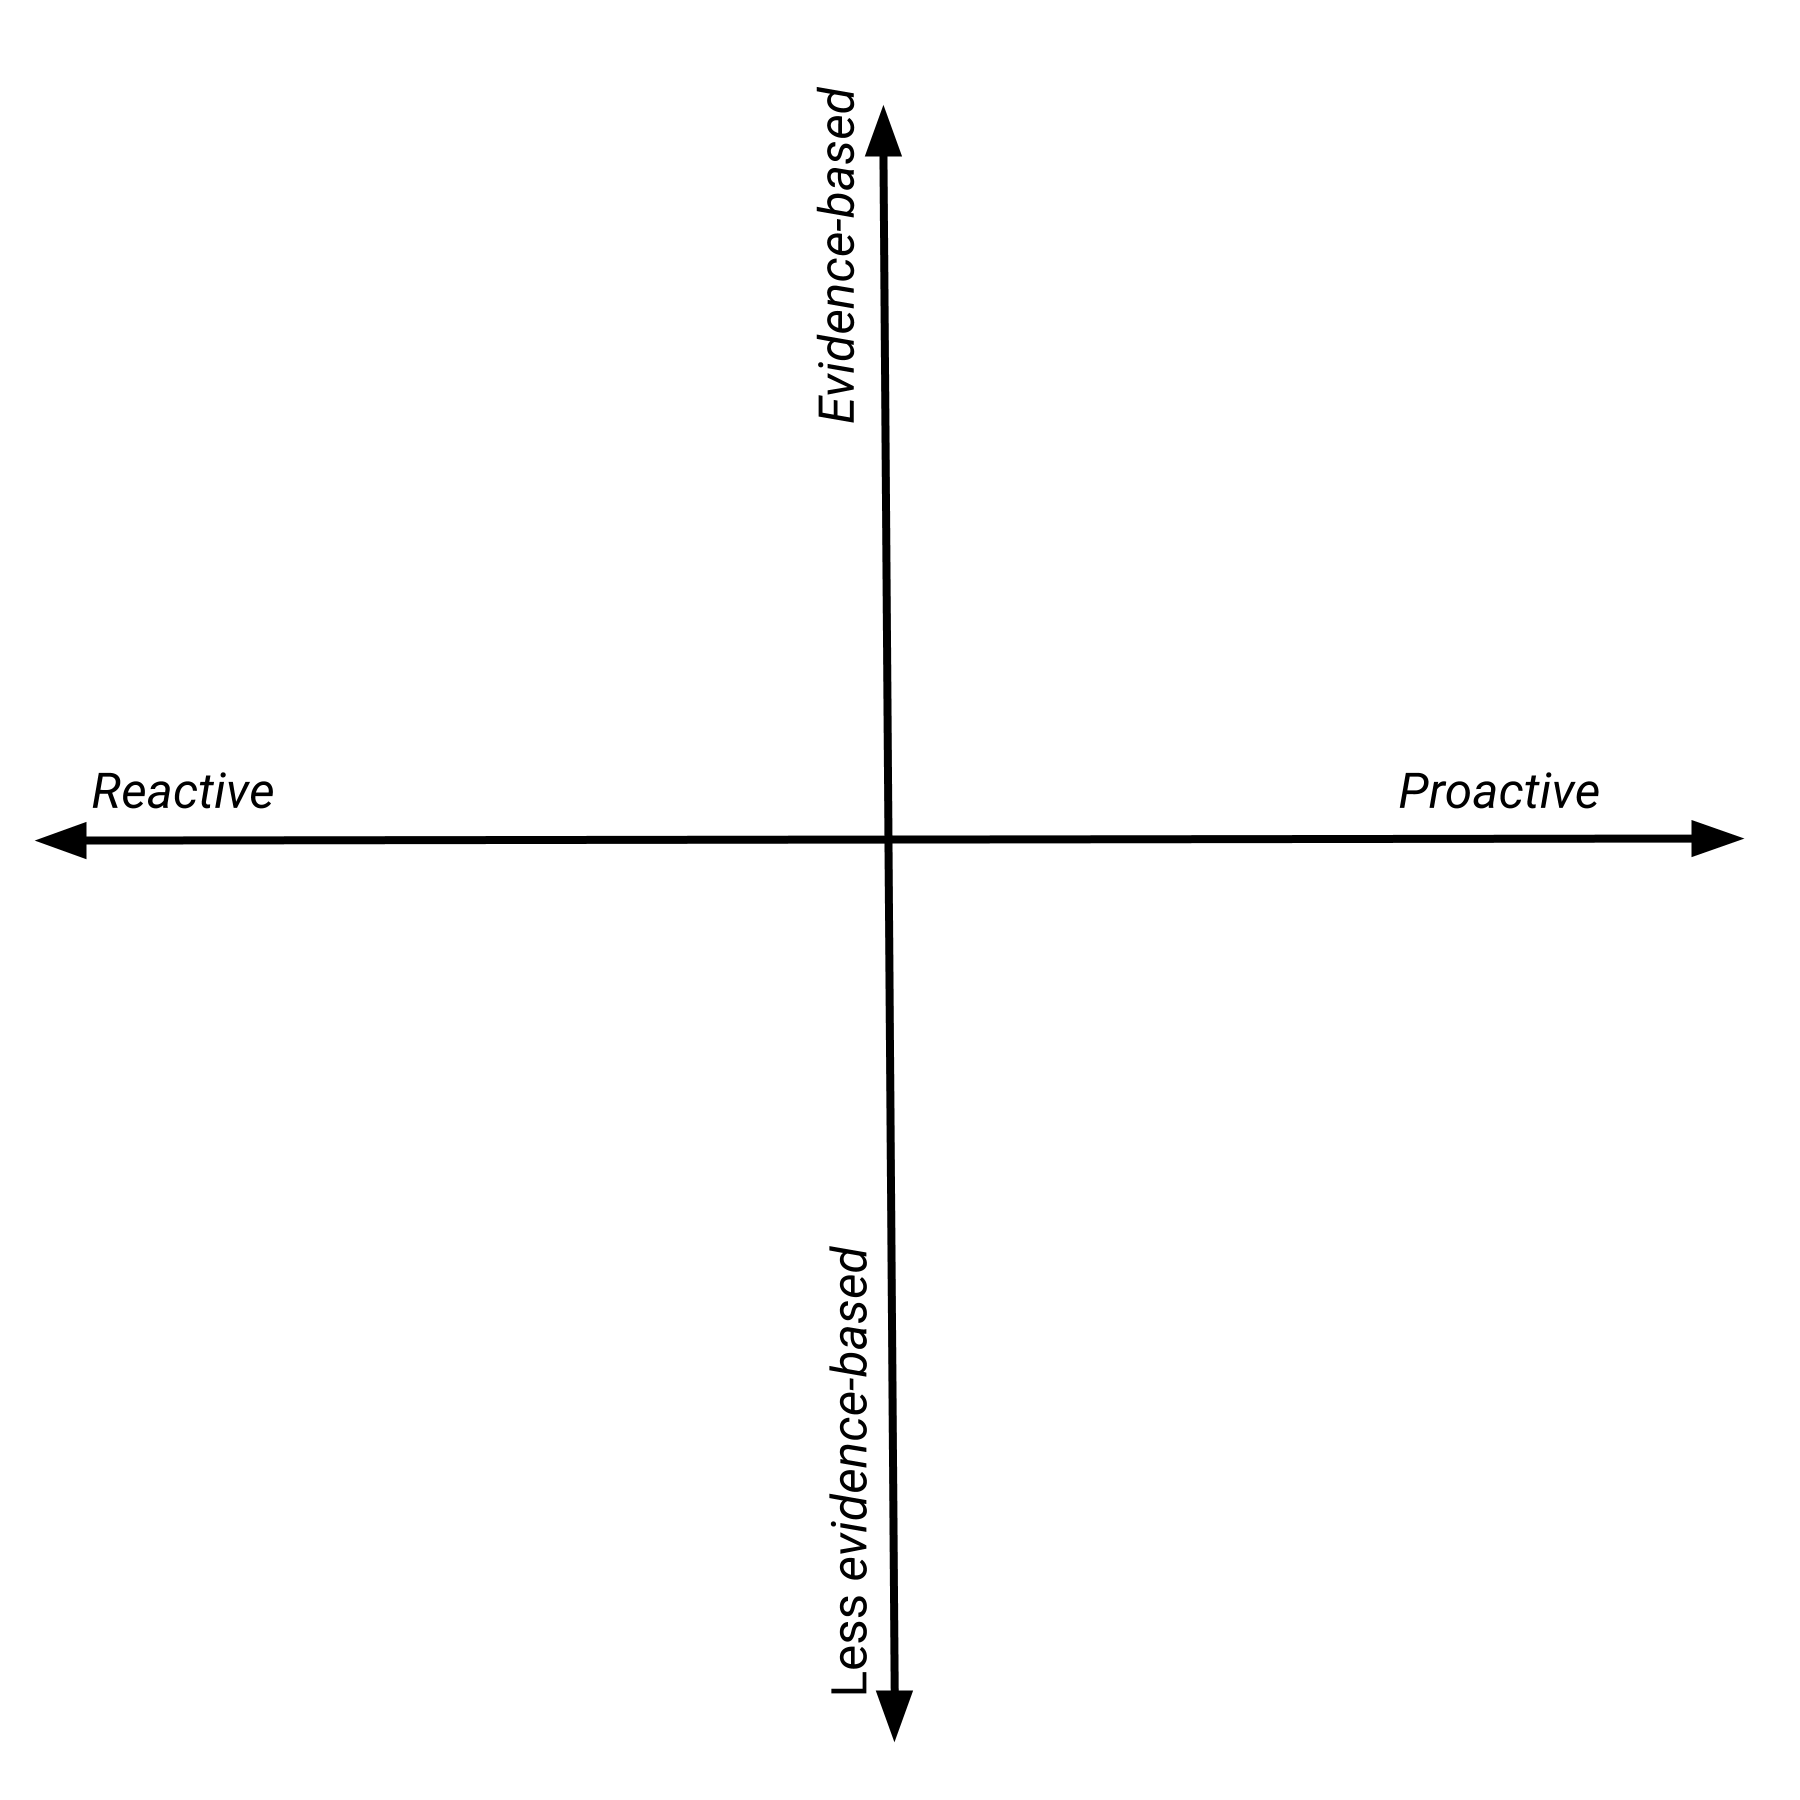
\includegraphics[width=0.65000\textwidth]{files/CMEthics_context3.png}
\caption{image}
\end{figure}

\subsection{Theme 3: Navigating practice in a retail
environment}\label{theme-3-navigating-practice-in-a-retail-environment}

I own a pharmacy \ldots{} I still work in the shop on a daily basis. So
I still come across on a daily basis having to chat to people about
this. But them I am also going to come at it from the side {[}that
\textbf{complementary medicines}{]} \textbf{prop up half of the bank
loan}. (D5P7)

If a pharmacy's going to lose money for the sake of a sale, that isn't a
good enough reason for the sake of giving something out. We should
always be having a look at evidence-based treatments, \ldots{} (D4P5)

\subsection{Acceptability \&
feasibility}\label{acceptability-feasibility}

\begin{figure}
\centering
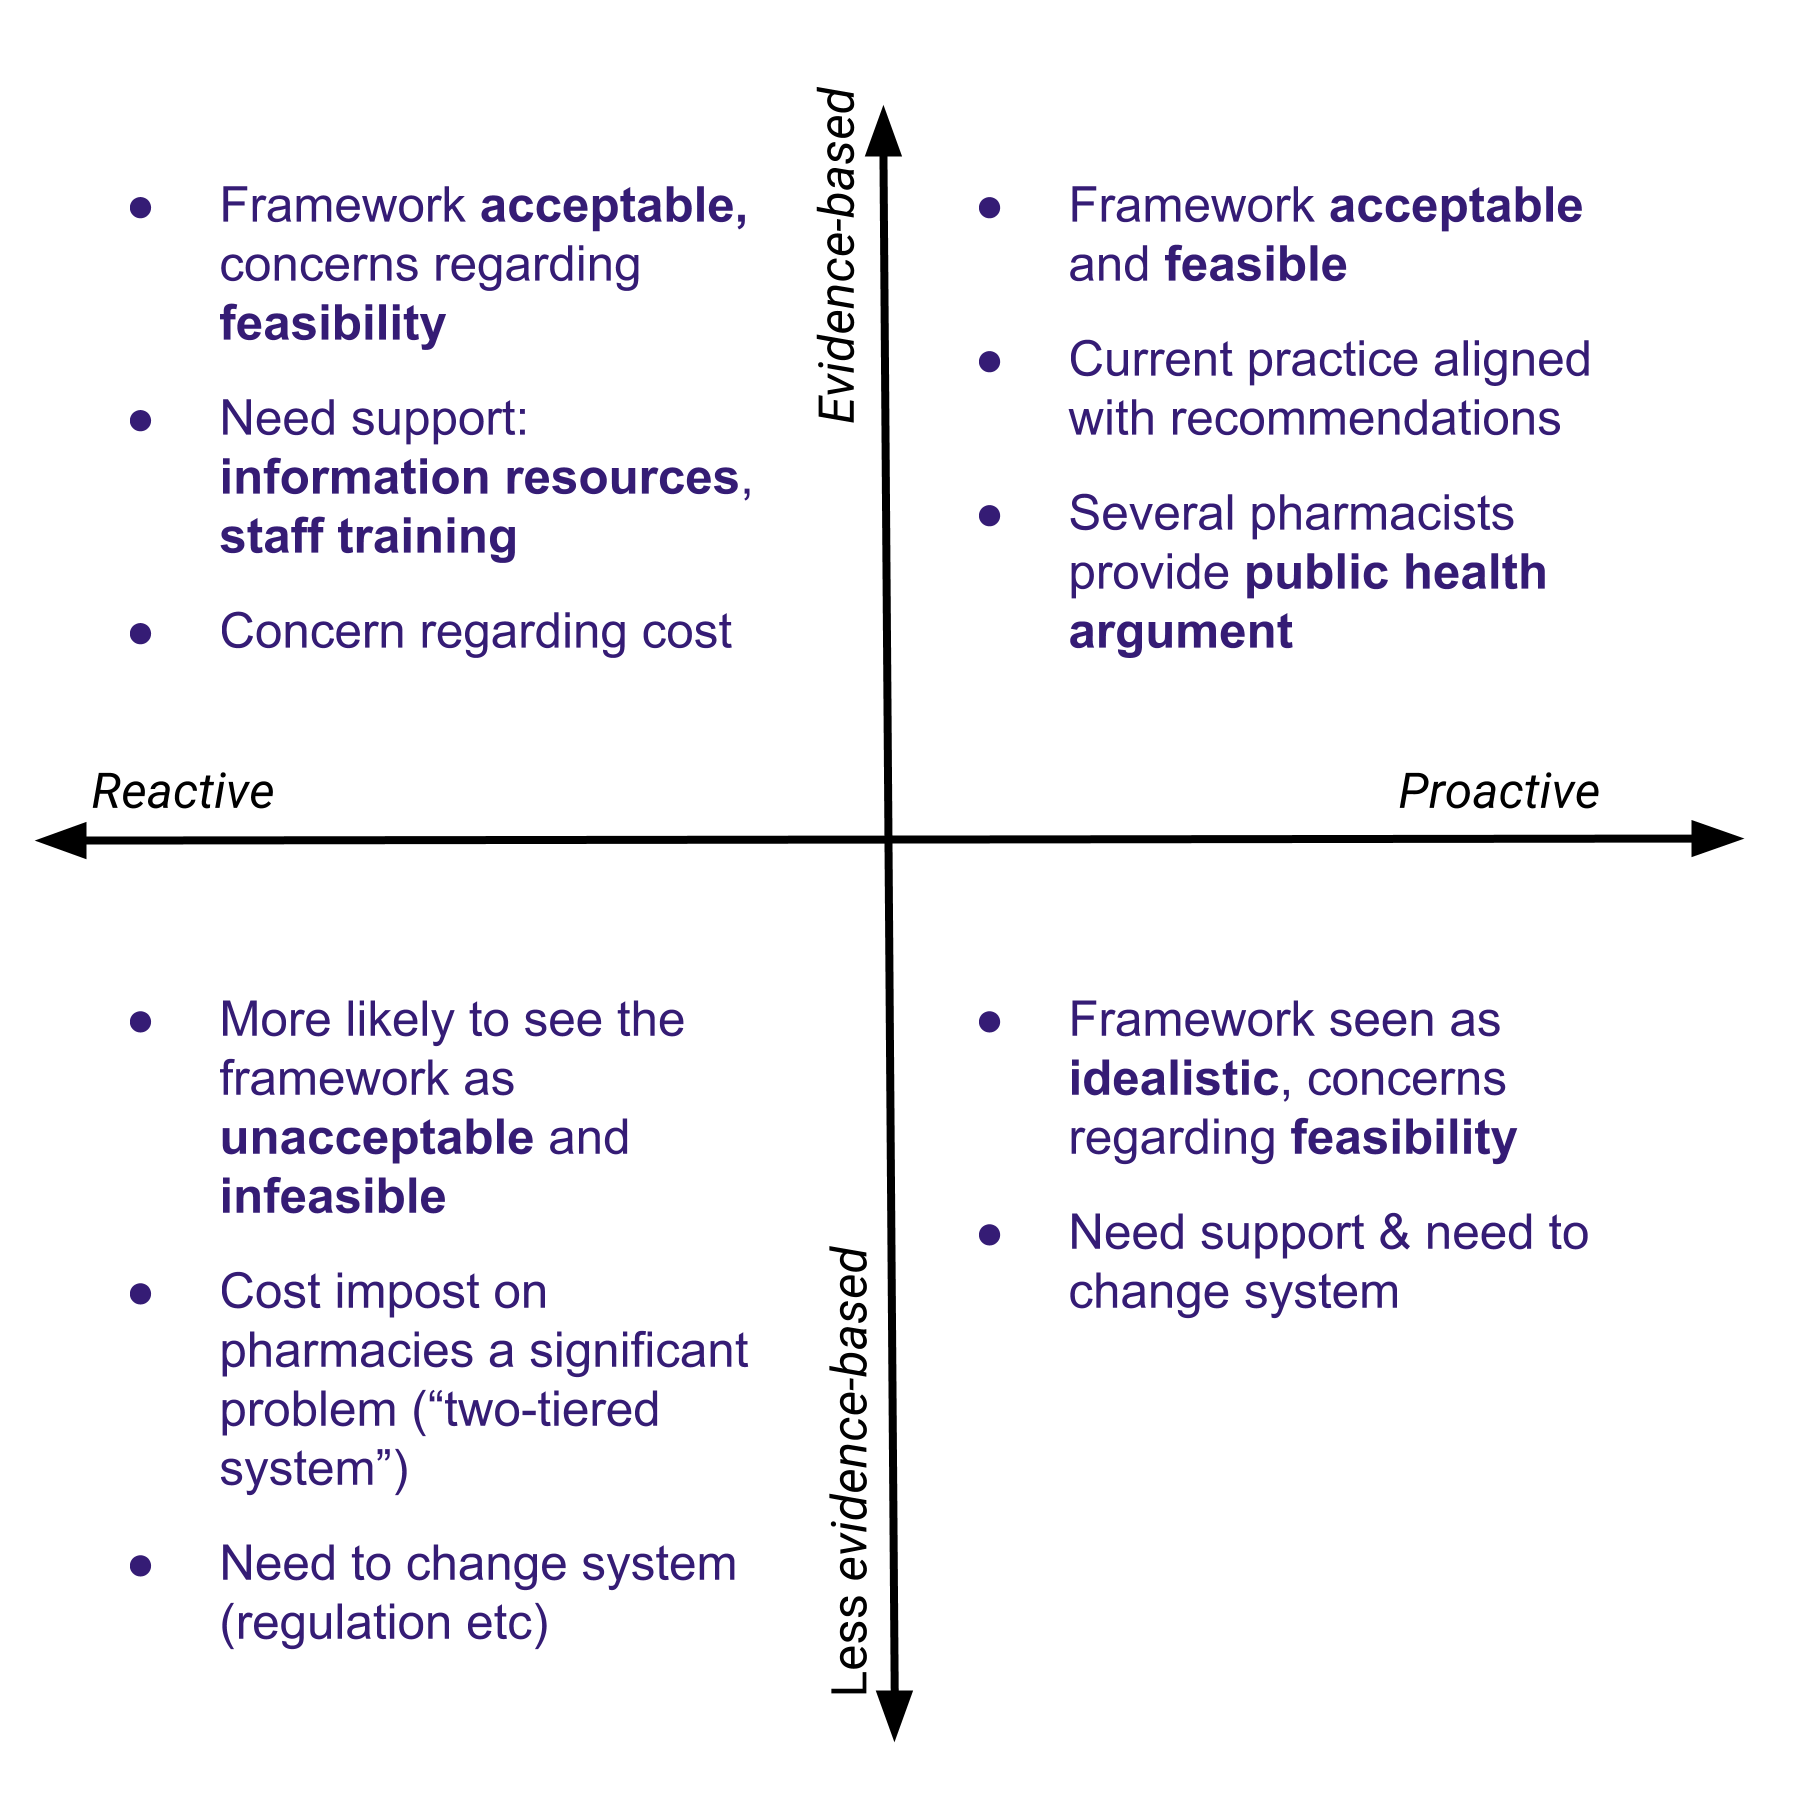
\includegraphics[width=0.65000\textwidth]{files/CMEthics_accfeas.png}
\caption{image}
\end{figure}

\subsection{Conclusion \& next steps}\label{conclusion-next-steps}

\begin{itemize}
\item
  The \emph{Framework for pharmacist responsibilities when selling
  complementary medicines} provides specific guidance to pharmacists on
  fulfilling their responsibilities when selling complementary medicines
\item
  The framework is \textbf{acceptable} to pharmacists and most felt it
  was \textbf{feasible}---especially with targeted support
\item
  The framework and findings of this study will be submitted to key
  professional professional bodies with the aim of informing policy
\end{itemize}

\subsection{Thanks \& questions}\label{thanks-questions}

\emph{Acknowledgements}

\begin{itemize}
\tightlist
\item
  This work was supported by an APSA Research Grant
\item
  Without this support it would not have been completed (yet)
\item
  Thank you to the professional services pharmacist that distributed the
  project invitation to their colleagues
\end{itemize}

\emph{Questions}

\begin{itemize}
\tightlist
\item
  \protect\hyperlink{ux2fthemes-common-topics-back}{Themes \& common
  topics}
\item
  \protect\hyperlink{ux2facceptability-cost-impost}{Quotes regarding
  cost impost}
\item
  \protect\hyperlink{ux2fadditional-threats-to-acceptability}{Additional
  threats to acceptability}
\item
  \protect\hyperlink{ux2fpsa-code-of-ethics}{PSA Code of Ethics
  guidance}
\item
  \protect\hyperlink{ux2freferences}{References}
\end{itemize}

\subsection{\texorpdfstring{Themes \& common topics
(\protect\hyperlink{ux2fthanks-questions}{Back})}{Themes \& common topics (Back)}}\label{themes-common-topics-back}

\begin{figure}
\centering
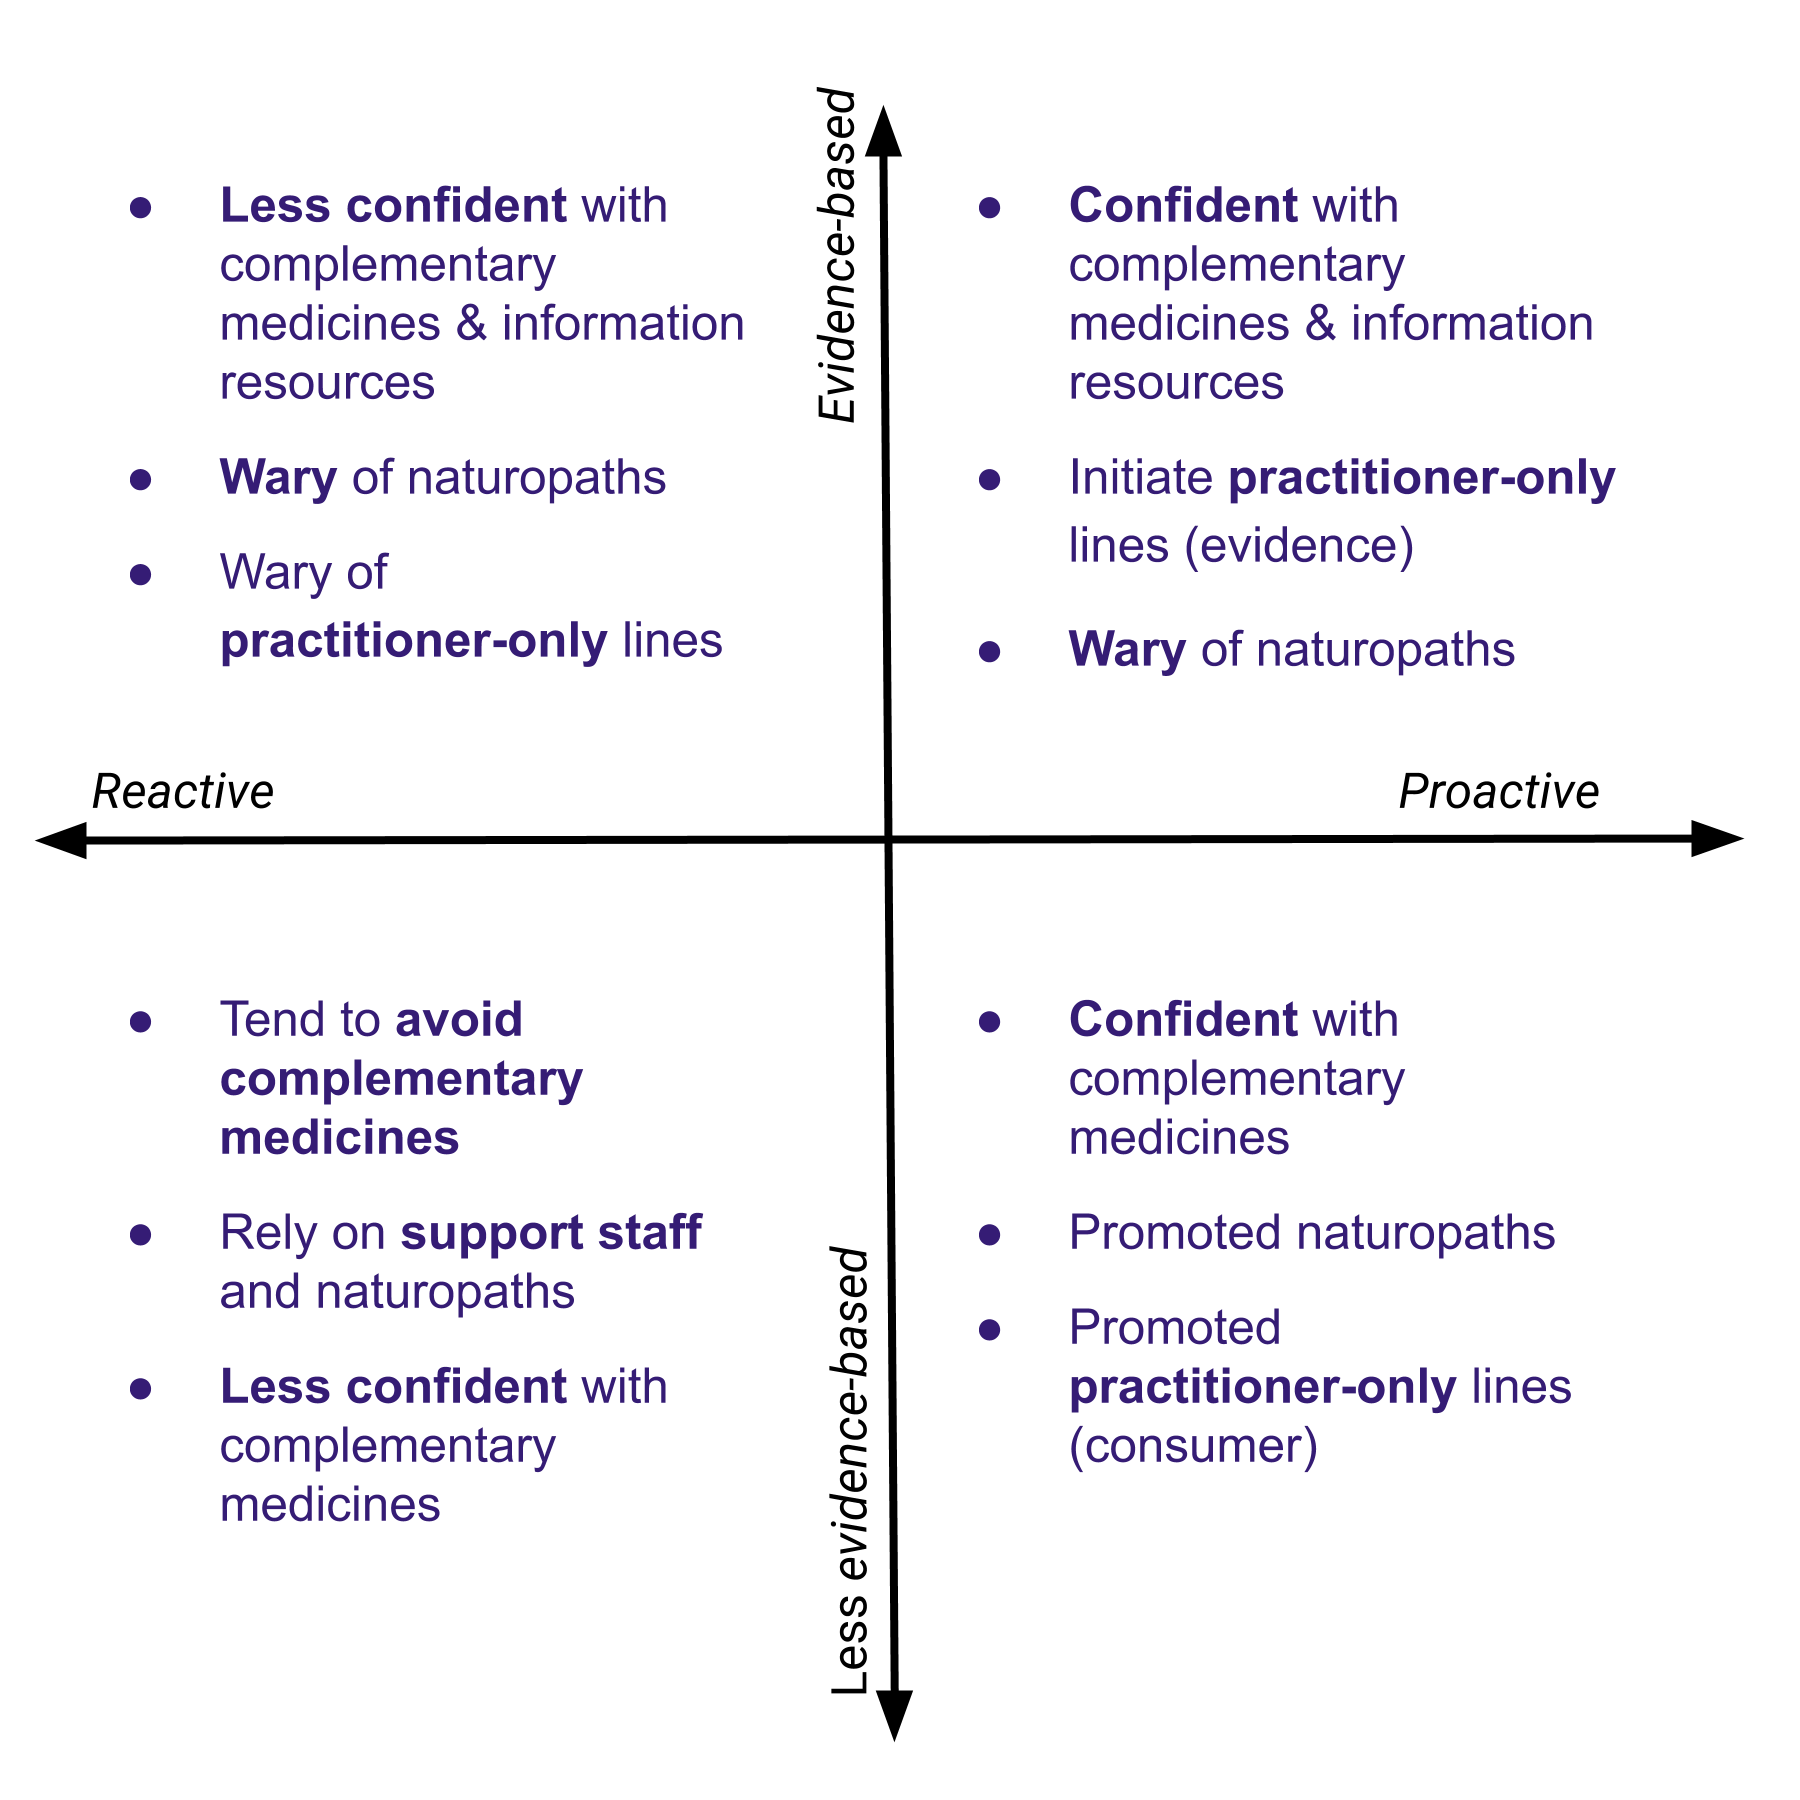
\includegraphics[width=0.65000\textwidth]{files/CMEthics_context2.png}
\caption{image}
\end{figure}

\subsection{Acceptability \& cost
impost}\label{acceptability-cost-impost}

I would say consumers mostly view {[}complementary medicines{]} as an
\textbf{item of commerce}. You buy them like you buy bread and milk, in
some instances, for some of them. So you've now imposed this cost on us
providing evidence, but in order to do that, we have to mark the product
up more. Then you've got this \textbf{two-tiered system}. (D5P7)

I think that having the degree means that \ldots{} people come for a
\textbf{higher level of service} and understanding than what they can
get in the supermarket. And that's part of what differentiates us
professionally. And that's part of why it's still called \textbf{a
pharmacy and not a supermarket}. I'm comfortable that I would actually
be probably more comfortable practising where the TGA just says, ``Yes,
that is safe to take.'' And then the pharmacist makes the clinical
judgement and says, ``Well, this may not be the best product for you.''
I think that that's literally our goal. (D5P9)

\protect\hyperlink{ux2fthanks-questions}{Back}

\subsection{Additional threats to
acceptability}\label{additional-threats-to-acceptability}

\begin{enumerate}
\def\labelenumi{\arabic{enumi}.}
\item
  Need to have a clear account of evidence-based practice in this
  context
\item
  Need to address arguments that the framework \textbf{doesn't go far
  enough}: imprimatur of selling complementary medicines; implicit
  recommendations (shelf-talkers, etc)
\end{enumerate}

\protect\hyperlink{ux2fthanks-questions}{Back}

\subsection{PSA Code of Ethics}\label{psa-code-of-ethics}

Integrity Principle 1 (h)

A pharmacist will only purchase, supply or promote any medicine,
complementary medicine, herbal remedy or other healthcare product where
there is credible evidence of efficacy and that benefit of use outweighs
the risk

\protect\hyperlink{ux2fthanks-questions}{Back}

\subsection{References}\label{references}

\printbibliography[heading=none]


\end{document}